Reinforcement Learning (RL) is an area of machine learning that studies how an agent interacts with an environment receiving instant rewards \cite{Sutton1998}.
The standard RL setup consists of an agent interacting with an environment $E$ in discrete timesteps. 
At each timestep $t$, an agent receives an observation $S_t$, takes action $A_t$ and ends up in state $S_{t+1}$, receiving an 
scalar reward $R_{t+1}$.
Figure \ref{fig:RL_image} illustrates this notion.

\begin{figure}[b]
    \centering
    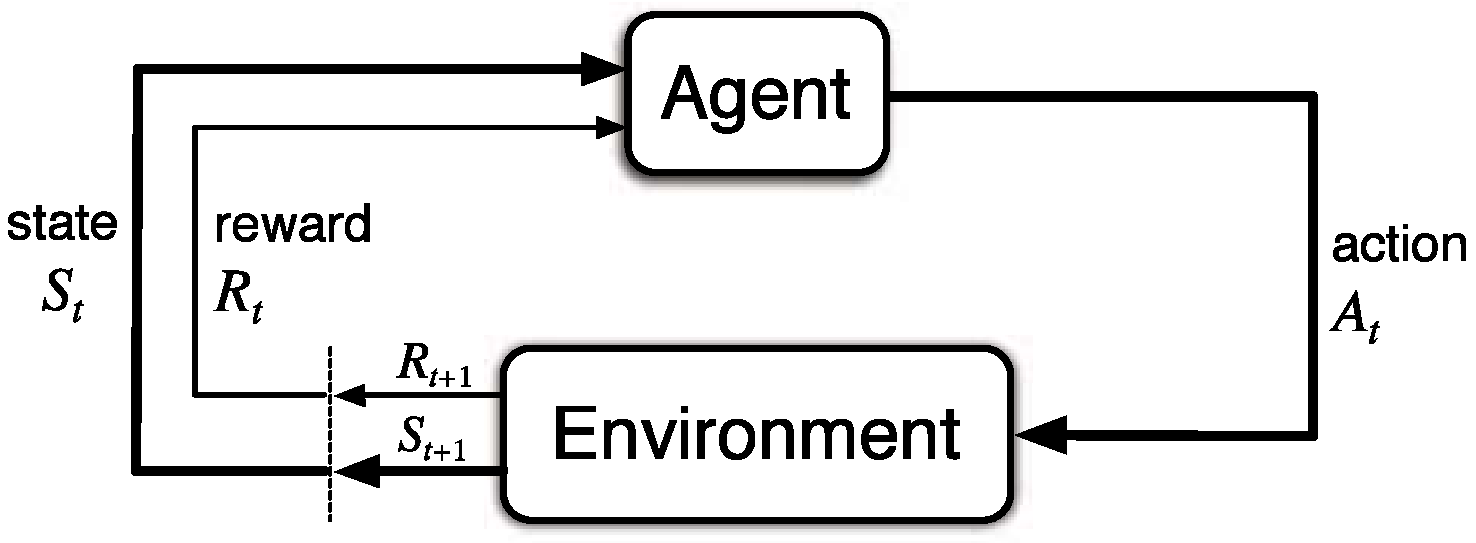
\includegraphics[width=0.8\textwidth]{Chapter2/RL_image.pdf} 
    \caption{Agent interacting with environment.}
    \label{fig:RL_image}
\end{figure}

RL is a simple yet powerful framework that defines the interaction between the agent and the environment. 
The agent learns from the environment in order to achieve long-term goals.

When modelling a problem with RL, there are 3 main components that must be carefully modeled:

\begin{itemize}
    \item \textbf{State space}: set of values that define the state of the agent in the environment.
    This represents the information available to the agent.
    \item \textbf{Action space}: set of values that define the possible actions the agent can take in the environment.
    \item \textbf{Reward signal}: defines how the agent is rewarded in regards to the goal.
\end{itemize}

The agent's goal is to maximize the cumulative reward it gets when interacting with the environment.
Note that normally these interactions are episodic, which means that the task restarts after some number of steps.

The following sections will describe the theory behind RL.

\section{Markov Decision Process}

A Markov Decision Processes (MDP) defines a mathematical framework that formally describes this interaction with the environment.
It is said that if the state of the agent contains all the necessary information from the past, it has the Markov Property and can be defined formally as:

\begin{equation}
    \mathcal{P}(S_{t + 1} | S_t) = \mathcal{P}(S_{t + 1} | S_1, S_2, ..., S_t)
\end{equation}

Therefore, a RL problem is an MDP if it has the Markov Property.

A particular MDP is defined by

\begin{itemize}
    \item State set, $\mathcal{S}$.
    \item Action set, $\mathcal{A}$.
    \item Initial state distribution $P(S_1)$.
    \item One-step transition dynamics of the environment $E$, denoted as $\mathcal{P}(S_{t+1} | S_t, A_t)$.
\end{itemize}

In general, the environment may be partially observed so that the entire history of state-action pairs
would be required to fully describe the state. 

\section{Return}

The return from state $S$ is defined as the sum of discounted future reward from timestep $t$:

\begin{equation}
    G_t = R_{t +1} + \gamma R_{t + 2} + ... = \sum_{k = 0}^{\infty}\gamma^k R_{t + k + 1}
\end{equation}

Notice that $\gamma \in [0,1]$ introduces the concept of discounting so that the agent prefers to gain instant rewards instead of long term rewards.
Also, the return depends on the actions being chosen (therefore on the policy $pi$ as well) and may be stochastic.

\section{Policies}

A policy $\pi$ maps the states to a probability distribution over the actions $\pi: \mathcal{S} \rightarrow \mathcal{P}(\mathcal{A})$.
It is represented by Equation \eqref{eq:policy}.

\begin{equation}
    \pi(a|s) = \mathcal{P}[A_t = a \vert S_t = s]
    \label{eq:policy}
\end{equation}

The policy fully describes the behavior of the agent and can also be deterministic formalized as
$\mu_\theta : \mathcal{S} \rightarrow \mathcal{A}$ with parameter vector $\theta \in  \mathbb{R}^2$ and
$A_t$ = $\mu_\theta(S_t)$.

\section{Value functions}

The value functions are estimates of the agent's current return.

\begin{itemize}
    \item State-value function 
    \begin{equation}
        v_\pi(s) = \mathbb{E}[G_t \vert S_t = s]
    \end{equation}

    \item Action-value function
    \begin{equation}
        q_\pi(s, a) = \mathbb{E}[G_t \vert S_t = s, A_t = a]
    \end{equation}
\end{itemize}

The value function estimates how good the agent's current state is (or how good it is for it to take a given action at that state).

\section{Goal of RL}

The goal of RL is to learn the optimal behavior (described by the policy) of the agent. This policy maximizes
the expected return $\mathbb{E}_{R_i, S_i \sim E, A_i \sim \pi} [G_1]$.
We will now define optimality for the value function and policy:

\subsection{Optimal Value Function}

The value functions are optimal if they are the highest value for all states (or state-action pairs).

\begin{itemize}
    \item Optimal State-value function: $v_*(s) = \underset{\pi}{\textrm{max }} v_\pi(s)$.
    \item Optimal Action-value function: $q_*(s, a) = \underset{\pi}{\textrm{max }} q_\pi(s, a)$.
\end{itemize}

Therefore, solving an MDP means finding the optimal value function (or optimal policy).

\subsection{Optimal Policy}

Let the partial ordering of policies be

\begin{align*}
    \pi \geq \pi\prime \text{ if } v_\pi(s) \geq v_{\pi\prime}(s)
\end{align*}

The optimal policy is better than any other,  $\pi_* \geq \pi, \forall \pi$ and achieves the optimal value functions.

An interesting property of the optimal policy is that it can be implicitly defined with $q_*$.
The optimal policy can be defined as the following deterministic policy

\[
    \pi_*(a | s) = 
\begin{cases}
    1,& \text{if } a = \underset{a'}{\textrm{argmax }} q_*(s,a')\\
    0,& \text{otherwise}
\end{cases}
\]

\section{Function Approximation}

Many classic tabular RL algorithms work by estimating the value functions for each state, for example, Value Iteration methods.
A problem arises when the state/action spaces are extremely large, or if the state/action spaces are continuous.
Some examples of large discrete state spaces are board games. This is known as the \textit{curse of dimensionality} \cite{CurseOfDimensionality}.
Backgammon has over $10^{20}$ board states \cite{Backgammon} and the game of Go (with board size of 19x19) has over $10^{170}$ states \cite{GoGame}. 
Figure \ref{fig:games} illustrates these games.

\begin{figure}[ht]
    \centering
   \begin{subfigure}[b]{0.45\textwidth}
            \centering
           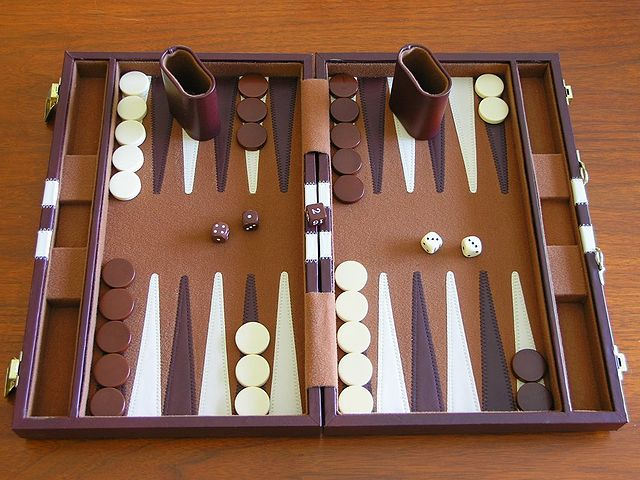
\includegraphics[height=0.75\textwidth]{Chapter2/backgammon_board.jpg}
           \caption{Game of Backgammon.}
   \end{subfigure}
   ~~
    \begin{subfigure}[b]{0.45\textwidth}
            \centering
            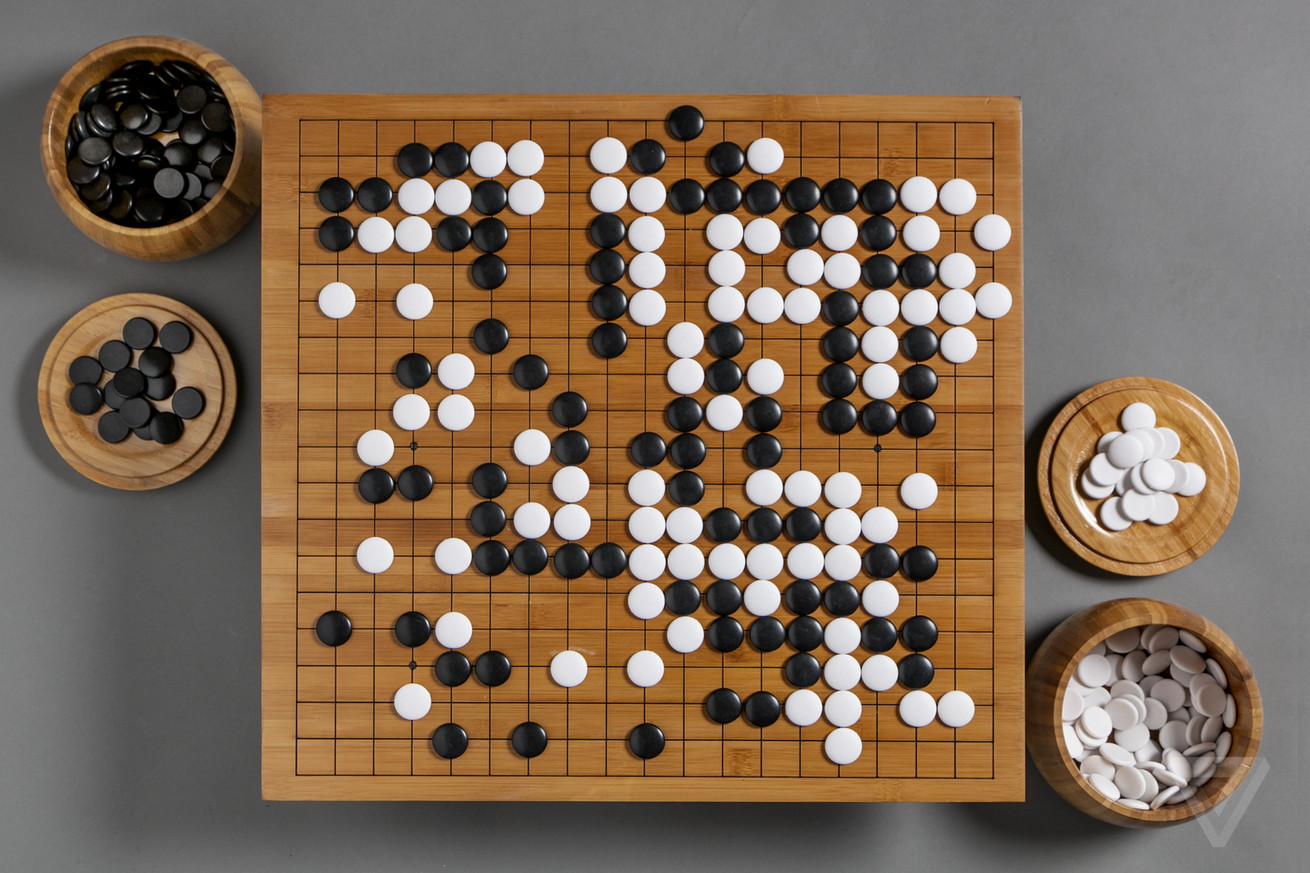
\includegraphics[height=0.75\textwidth]{Chapter2/go_board.png}
            \caption{Game of Go.}
   \end{subfigure}
   \caption{Example of board games that have large discrete state spaces.}
  \label{fig:games}
\end{figure}


There are 2 problems of having so many states in realistic situations:

\begin{itemize}
    \item It will be impossible to store all the states in memory.
    \item It will be impossible to visit all the states in training.
\end{itemize}
 
For continuous domains, we have an analogous situation since it is possible to discretize the state or action space and then apply tabular methods.
Figure \ref{fig:continuous} illustrates 3 continuous control problems and the number of states resulting from one possible discretization.

\begin{figure}[ht]
    \centering
    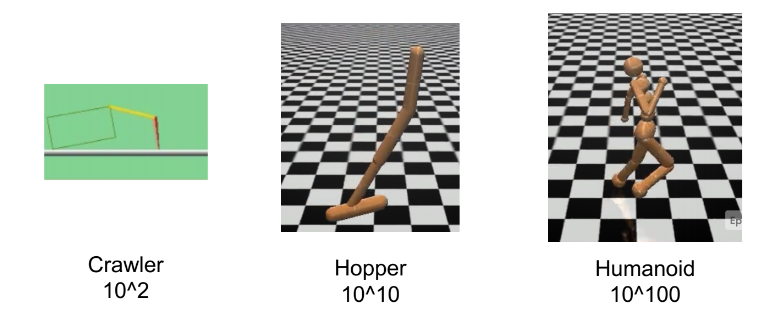
\includegraphics[width=1\textwidth]{Chapter2/continuous.png}
    \caption{Sample control tasks from the \cite{OpenAIGym} toolkit.}
  \label{fig:continuous}
\end{figure}

If the discretized space is large, we still have the problem described above.
An approach to deal with this problem is to use a function approximation that estimates the value function.
The approximate value function, $\hat{v}(s, \theta)$ will be defined by a parameter weight vector $\theta \in \mathbb{R}^n$ and

\begin{align*}
    \hat{v}(s, \theta) \approx v_\pi(s)
\end{align*}

The interesting part of function approximation is that this function estimator can be any function,
 ranging from a simple linear function of the states to a complex NNs.
Normally the number of weights is much less than the number of states.

In this work, we focused on using neural networks as function approximators; Chapter \ref{chap:deep_learning} lays
the groundwork for the theory regarding Neural Networks.

\section{RL algorithms}

There are 3 classes of RL algorithms: methods based on value functions, methods based on policy search and a hybrid approach
which combines value functions and policy search \cite{Sutton1998}.

\subsection{Value Function Methods}

Value function methods are based on estimating $v$ or $q$ functions.
Monte-Carlo (MC) methods and TD Learning are the two methods generally used for predicting the value function \cite{Sutton1998}.

\subsubsection{Monte-Carlo}

MC prediction are model-free (i.e. they do not require knowledge of the underlying dynamics) methods that learn directly from complete episodes of experience.
They estimate the value functions by averaging sample returns and therefore can only be applied to episodic MDPs.

\subsubsection{Temporal-Difference Learning}

TD Learning are model-free and can learn from incomplete episodes. TD Learning updates the estimate by \textit{bootstrapping}, which
means it updates the value function using an existing estimate.

The simplest TD method, known as TD($0$), updates the value function as

\begin{equation}
    V(S_t) = V(S_t) + \alpha [R_{t+1} + \gamma V(S_{t+1}) - V(S_t)]
    \label{eq:td_learning}
\end{equation}

TD has some advantages in comparison to MC: TD can learn before the end of that episode (or in non episodic MDPS) and have low variance and some bias.
MC on the other hand has high variance, zero bias, having good convergence properties (even with function approximation). 

\subsection{Policy Search Methods}

Policy search methods do not have an estimate of the value function. These algorithms typically maintain a parameterized policy $\pi_\theta$
whose parameters are updated to maximize the expected return.
The Policy Gradient Theorem defines that for any differentiable policy $\pi_\theta(s,a)$ the policy
gradient is

 \begin{equation}
     \nabla_\theta J(\theta) = \mathbb{E}_{\pi_\theta}[\nabla_{\pi_\theta} \log{\pi_\theta(s,a) Q^{\pi_\theta}(s,a)}]
     \label{eq:pg_theorem}
 \end{equation}

 An example usage of this theorem is seen in the REINFORCE algorithm that uses Equation \eqref{eq:pg_theorem}
 to update the policy's weight using gradient ascent \cite{REINFORCE}.

\subsection{Actor-Critic Methods}

Actor-critic methods also work by updating a parameterized policy $\pi_\theta$ but instead use a \textit{critic}
to estimate the action-value function \(Q^{\pi_\theta}\),

\[
 Q_w(s,a) \approx Q^{\pi_\theta}(s,a)
\]

where \(w\) is the weight vector that parameterizes $Q$. Therefore actor-critic algorithms maintain two
sets of parameters: the \textit{critic} that updates that action-value function parameters \(w\) and
the \textit{actor} that updates the policy parameters \(\theta\) in the direction suggested by the \textit{critic}.

Figure \ref{fig:actor_critic} illustrates the architecture of actor-critic algorithms.

\begin{figure}[ht] 
    \centering
    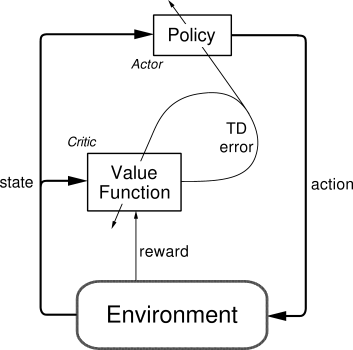
\includegraphics[width=0.6\textwidth]{Chapter2/actor_critic.png}
    \caption{Actor-critic architecture from \cite{Sutton1998}.}
  \label{fig:actor_critic}
\end{figure}

\section{Curriculum Learning}

Reinforcement learning has been used to solve non-trivial tasks in locomotion \cite{TRPO} and video games \cite{RLNature2015}.

However, there are many tasks that are hard to design a reward function that is easily maximized and that when optimized yields the expected behavior \cite{ReverseCurrLearning}.
For example, tasks with sparse rewards are still challenging since it is very hard to achieve the goal following random exploration \cite{TSCurrLearning}.
One approach to overcome this problem is to use curriculum learning \cite{BengioCurrLearning}.

Curriculum learning is a sequence of training criteria where tasks are ordered by increasing difficulty and training
moves from to a harder task only when it has mastered the easier tasks. 
Usually, to apply curriculum learning to a task, the researcher must be able to order the subtasks by difficulty and 
decide the heuristics for when a subtask has been mastered \cite{TSCurrLearning}.

Curriculum learning is a recent idea that has been applied to a wide range of RL problems. An interesting
result is \citen{ExecuteCurrLearning} that applies a variant of curriculum learning to evaluate short computer programs.
Some other examples include \cite{OpenAISelfPlay, TSCurrLearning}.
